% NeurIPS-style project report: GPTQ post-training quantization (TinyLlama).
% -----------------------------------------------------------------------------
% Build (from this directory):
%   pdflatex main
%   bibtex main
%   pdflatex main
%   pdflatex main
%
% Official style: download \texttt{neurips\_2024.sty} from the NeurIPS author
% kit (\url{https://neurips.cc/Conferences/2024/CallForPapers}) and place it
% next to \texttt{main.tex}. If the file is missing, this template falls back to
% a compact \texttt{article} layout with similar margins.
% -----------------------------------------------------------------------------

\documentclass[11pt]{article}

\usepackage[utf8]{inputenc}
\usepackage[T1]{fontenc}

\IfFileExists{neurips_2024.sty}{%
  \usepackage[preprint, nonatbib]{neurips_2024}
}{%
  \usepackage[margin=1in]{geometry}
  \usepackage{times}
  \usepackage{helvet}
  \usepackage{courier}
  \sloppy
}

\usepackage{microtype}
\usepackage[numbers,sort&compress]{natbib}
\usepackage{xcolor}
\usepackage{graphicx}
\usepackage{booktabs}
\usepackage{amsmath}
\usepackage{amssymb}
\usepackage{url}
\usepackage{hyperref}
\hypersetup{
  colorlinks=true,
  linkcolor=blue,
  citecolor=blue,
  urlcolor=blue,
}

% Placeholder macro for CSV-filled table cells (replace with real numbers).
\newcommand{\placeholder}[1]{\textcolor{gray}{\textit{[\,#1\,]}}}

\graphicspath{{../results/figures/}{figures/}}

\title{Post-Training Quantization for Small Language Models: \\
  GPTQ-Centric Evaluation with Optional AWQ on TinyLlama}

\author{%
  Team Name / Author List Placeholder\\
  Institution Placeholder\\
  \texttt{email@institution.edu}
}

\begin{document}
\maketitle

\begin{abstract}
We study \emph{post-training quantization} (PTQ) for decoder-only language models at the $\sim$1B parameter scale.
Using \textbf{TinyLlama-1.1B-Chat} as a representative small model, we implement and compare three primary regimes:
full-precision FP16, GPTQ 4-bit, and GPTQ 3-bit weight-only quantization.
AWQ 4-bit is treated as an optional extension because some Windows + \texttt{transformers==4.37.2}
environments cannot import AutoAWQ reliably.
All methods are evaluated under a unified Windows + NVIDIA CUDA pipeline with consistent calibration data (WikiText-2),
open toolchains (\texttt{AutoGPTQ}, optional \texttt{AutoAWQ}), and shared prompts for timing.
We report \textbf{WikiText-2 perplexity}, \textbf{greedy decoding throughput}, and \textbf{peak GPU memory}
from PyTorch's CUDA allocator.
Empirically, aggressive 3-bit GPTQ achieves the smallest footprint but often degrades perplexity relative to 4-bit methods.
When AWQ runs are available, they provide an additional accuracy--efficiency comparison point.
We release scripts, CSV logs, and publication-style figures to support reproducibility.
\end{abstract}

\section{Introduction}
Large language models (LLMs) have become the workhorse of modern NLP, but their memory and compute costs limit
deployment on single-GPU workstations and edge servers.
\emph{Quantization} reduces the bit-width of weights (and sometimes activations), shrinking model size and
accelerating matrix multiplications on hardware that supports low-bit kernels.

This project focuses on \textbf{post-training quantization}: we start from a pretrained checkpoint and calibrate
quantizers using a small unlabeled text corpus, \emph{without} end-to-end retraining.
We target \textbf{TinyLlama}~\citep{zhang2024tinyllama}, a compact open model suited to rapid experimentation,
and compare:
(i) FP16 baseline,
(ii) GPTQ 4-bit and 3-bit~\citep{frantar2023gptq},
with optional AWQ 4-bit runs when environment compatibility permits~\citep{lin2023awq}.

\textbf{Contributions.}
\begin{itemize}
  \item A reproducible benchmarking harness (quantization, perplexity, speed, memory, plotting) on Windows + CUDA.
  \item Side-by-side evaluation of GPTQ (multiple bit-widths) on TinyLlama with WikiText-2 perplexity,
    plus optional AWQ comparisons when available.
  \item Analysis of the accuracy--speed--memory trade-offs at the 1B scale, with emphasis on practical pitfalls
    (calibration size, kernel backends, allocator statistics).
\end{itemize}

\section{Related Work}
\paragraph{Post-training quantization.}
PTQ methods compress pretrained weights using calibration batches to estimate scales and, for some algorithms,
higher-order statistics of activations.
GPTQ~\citep{frantar2023gptq} approximates the Hessian of the quantization objective layer-wise and has become a
standard for 3--4 bit weight-only compression of LLMs.
Prior work on mixed-precision and outlier handling (e.g., LLM.int8())~\citep{dettmers2022llmint8} motivates
separating outliers from bulk weights; GPTQ and AWQ can be viewed as complementary lines that emphasize
efficient layer-wise solvers and activation-aware scaling, respectively.

\paragraph{Activation-aware weight quantization (AWQ).}
AWQ~\citep{lin2023awq} protects ``salient'' weights by exploiting activation statistics, often improving robustness
at 4-bit precision relative to purely weight-space PTQ.
In practice, both GPTQ and AWQ rely on vendor- and library-specific CUDA kernels; our study reflects
\texttt{AutoGPTQ}~\citep{pan2024autogptq} and \texttt{AutoAWQ}~\citep{hansen2024autoawq} as shipped on PyPI.

\paragraph{Evaluation corpora.}
WikiText-2~\citep{merity2016pointer} remains a standard language modeling benchmark for perplexity comparisons;
we use the raw word-level split for calibration and evaluation consistency with common open implementations.

\section{Method}
\subsection{Base model and quantization targets}
We use \texttt{TinyLlama/TinyLlama-1.1B-Chat-v1.0} as the FP16 reference.
Chat-tuned checkpoints exhibit distributional shift relative to base LMs; we nevertheless use WikiText-2 for
\emph{comparability} with extensive prior work, noting that absolute perplexities must be interpreted relative to
the baseline rather than as state-of-the-art LM scores.

\subsection{GPTQ}
GPTQ minimizes layer-wise reconstruction error under integer constraints on weights, using second-order information
via a damped Hessian approximation~\citep{frantar2023gptq}.
We export 4-bit and 3-bit GPTQ checkpoints with group size $128$, no double quantization unless noted,
and WikiText-2 raw snippets for calibration (default: hundreds of short documents; exact $N$ logged in code).
\textbf{Triton-dependent} code paths are disabled on Windows; we rely on \texttt{AutoGPTQ}'s default CUDA kernels.

\subsection{AWQ (optional extension)}
AWQ performs 4-bit weight quantization with activation-aware protection of important channels~\citep{lin2023awq}.
We use the GEMM backend as exposed by \texttt{AutoAWQ}, with group size $128$ and zero-point quantization enabled,
matching library defaults documented for general LLaMA-family models.
Due to compatibility constraints on some Windows setups, AWQ runs may be omitted from the final benchmark tables;
the benchmark scripts are designed to continue gracefully in that case.

\subsection{Metrics}
\paragraph{Perplexity.}
For WikiText-2 test text, we report causal LM perplexity
$\mathrm{PPL} = \exp\bigl(-\tfrac{1}{T}\sum_{t}\log p_\theta(x_t \mid x_{<t})\bigr)$,
implemented with a sliding-window evaluation to avoid double-counting overlapped tokens (see project script documentation).

\paragraph{Throughput and latency.}
We measure wall time for greedy \texttt{generate} with \texttt{torch.cuda.synchronize()} brackets,
then compute tokens/s as (new tokens) / (elapsed time), averaging multiple iterations after warmup.

\paragraph{GPU memory.}
We report PyTorch \texttt{memory\_allocated}, \texttt{memory\_reserved}, and \texttt{max\_memory\_allocated}
around model load and a single generation, following the project's \texttt{benchmark\_memory.py} protocol.

\section{Experiments}
\subsection{Software and hardware}
\textbf{OS:} Windows 10/11.
\textbf{Python:} 3.10 (recommended for wheel compatibility).
\textbf{PyTorch:} CUDA 12.1 wheels; exact build recorded in project \texttt{README.md}.
\textbf{Libraries:} \texttt{transformers==4.37.2}, \texttt{auto-gptq==0.7.1}; \texttt{autoawq==0.2.5} is optional.
\textbf{Hardware placeholder:} NVIDIA GPU with \placeholder{XX}\,GB VRAM, driver version \placeholder{XXX}.

\subsection{Protocol}
\begin{enumerate}
  \item Quantize FP16 $\rightarrow$ GPTQ-4b and GPTQ-3b with fixed calibration sources.
  \item Optionally quantize AWQ-4b if AutoAWQ is available on the host.
  \item Evaluate WikiText-2 perplexity for each checkpoint (status=\texttt{ok} rows only).
  \item Benchmark greedy decoding speed with a \emph{shared} prompt and \texttt{max\_new\_tokens} held constant.
  \item Record peak allocator statistics after load and after one generation.
  \item Generate matplotlib figures (\texttt{scripts/generate\_graphs.py}) for the paper.
\end{enumerate}

\subsection{Results}
Table~\ref{tab:ppl} summarizes perplexity; Table~\ref{tab:speed} reports throughput and latency; Table~\ref{tab:memory}
summarizes GPU memory. Figures are loaded from
\texttt{results/figures/perplexity\_comparison.png},
\texttt{results/figures/inference\_speed.png}, and
\texttt{results/figures/memory\_usage.png}.

\begin{figure}[t]
  \centering
  \IfFileExists{../results/figures/perplexity_comparison.png}{%
    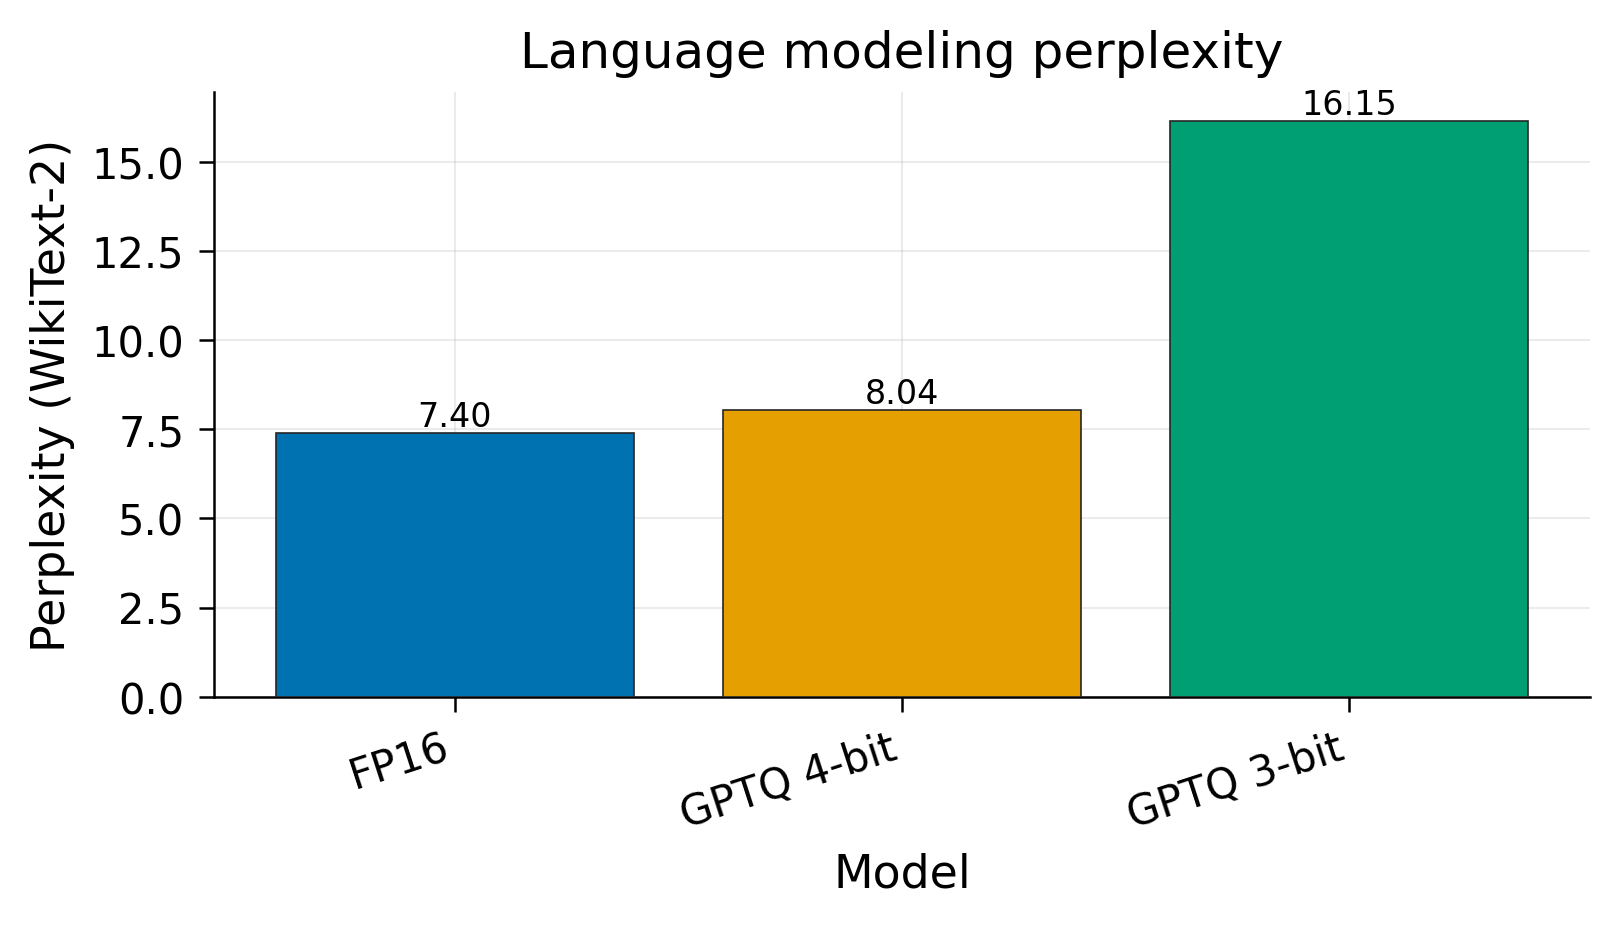
\includegraphics[width=0.85\linewidth]{perplexity_comparison.png}%
  }{%
    \fbox{\parbox[c][0.22\textheight]{0.85\linewidth}{\centering
      \vfill
      \textit{Placeholder: run \texttt{python scripts/generate\_graphs.py}\\
      to produce \texttt{results/figures/perplexity\_comparison.png}.}
      \vfill
    }}%
  }
  \caption{WikiText-2 perplexity comparison across FP16 and GPTQ variants (AWQ optional).}
  \label{fig:ppl}
\end{figure}

\begin{figure}[t]
  \centering
  \IfFileExists{../results/figures/inference_speed.png}{%
    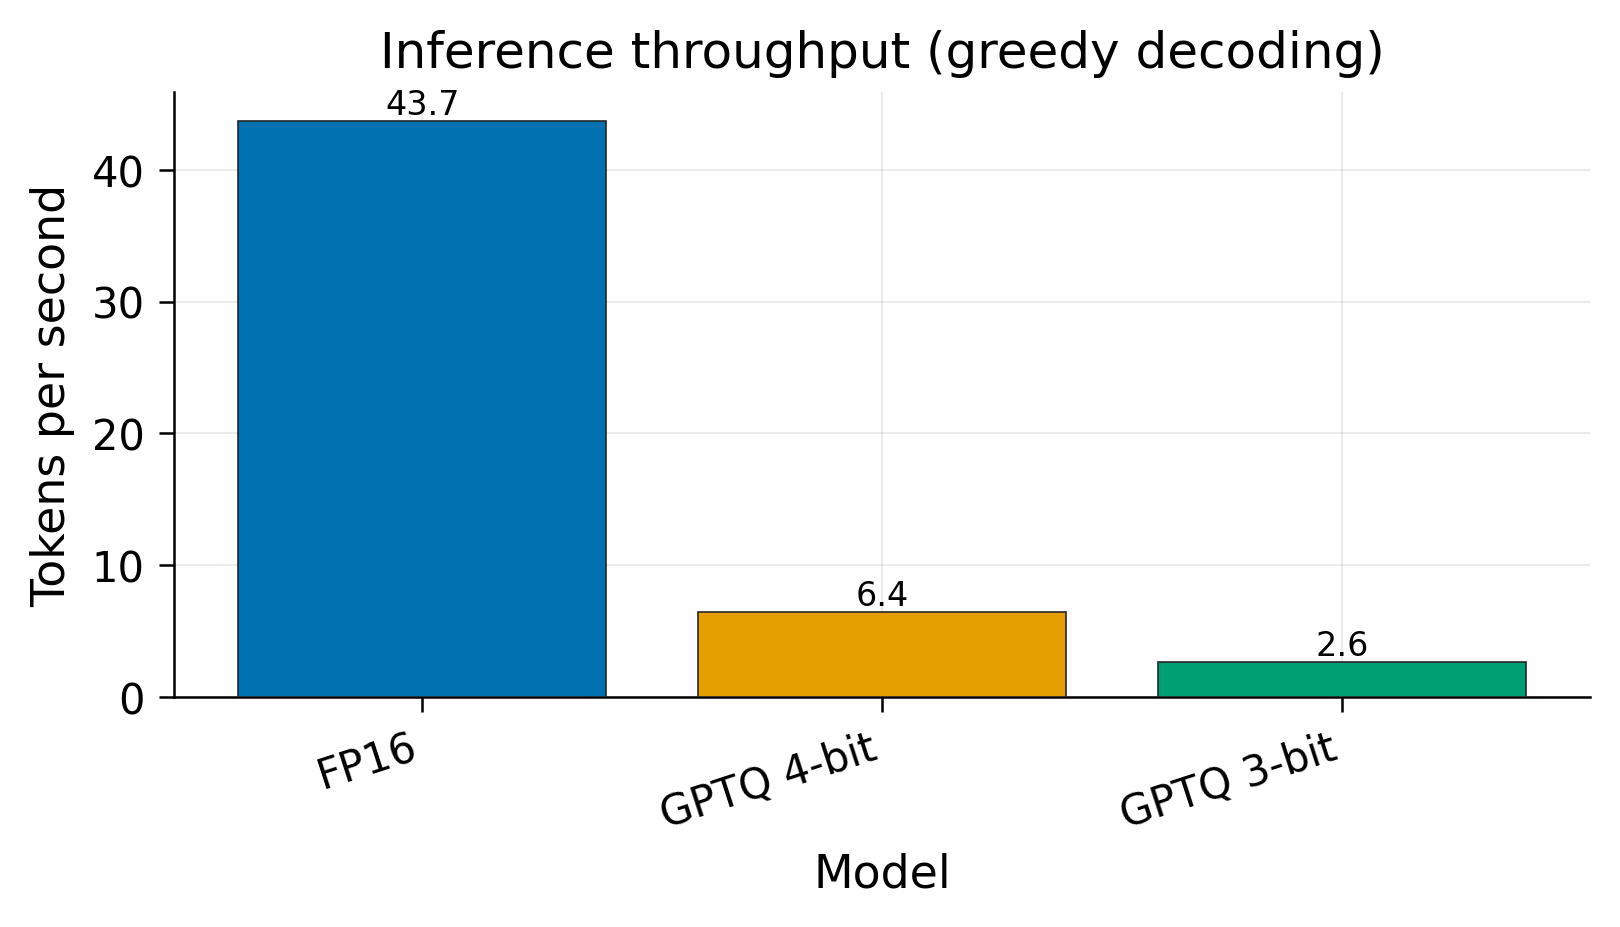
\includegraphics[width=0.85\linewidth]{inference_speed.png}%
  }{%
    \fbox{\parbox[c][0.22\textheight]{0.85\linewidth}{\centering
      \vfill
      \textit{Placeholder: \texttt{results/figures/inference\_speed.png}}
      \vfill
    }}%
  }
  \caption{Greedy decoding throughput (tokens/s) under a shared prompt and decoding budget.}
  \label{fig:speed}
\end{figure}

\begin{figure}[t]
  \centering
  \IfFileExists{../results/figures/memory_usage.png}{%
    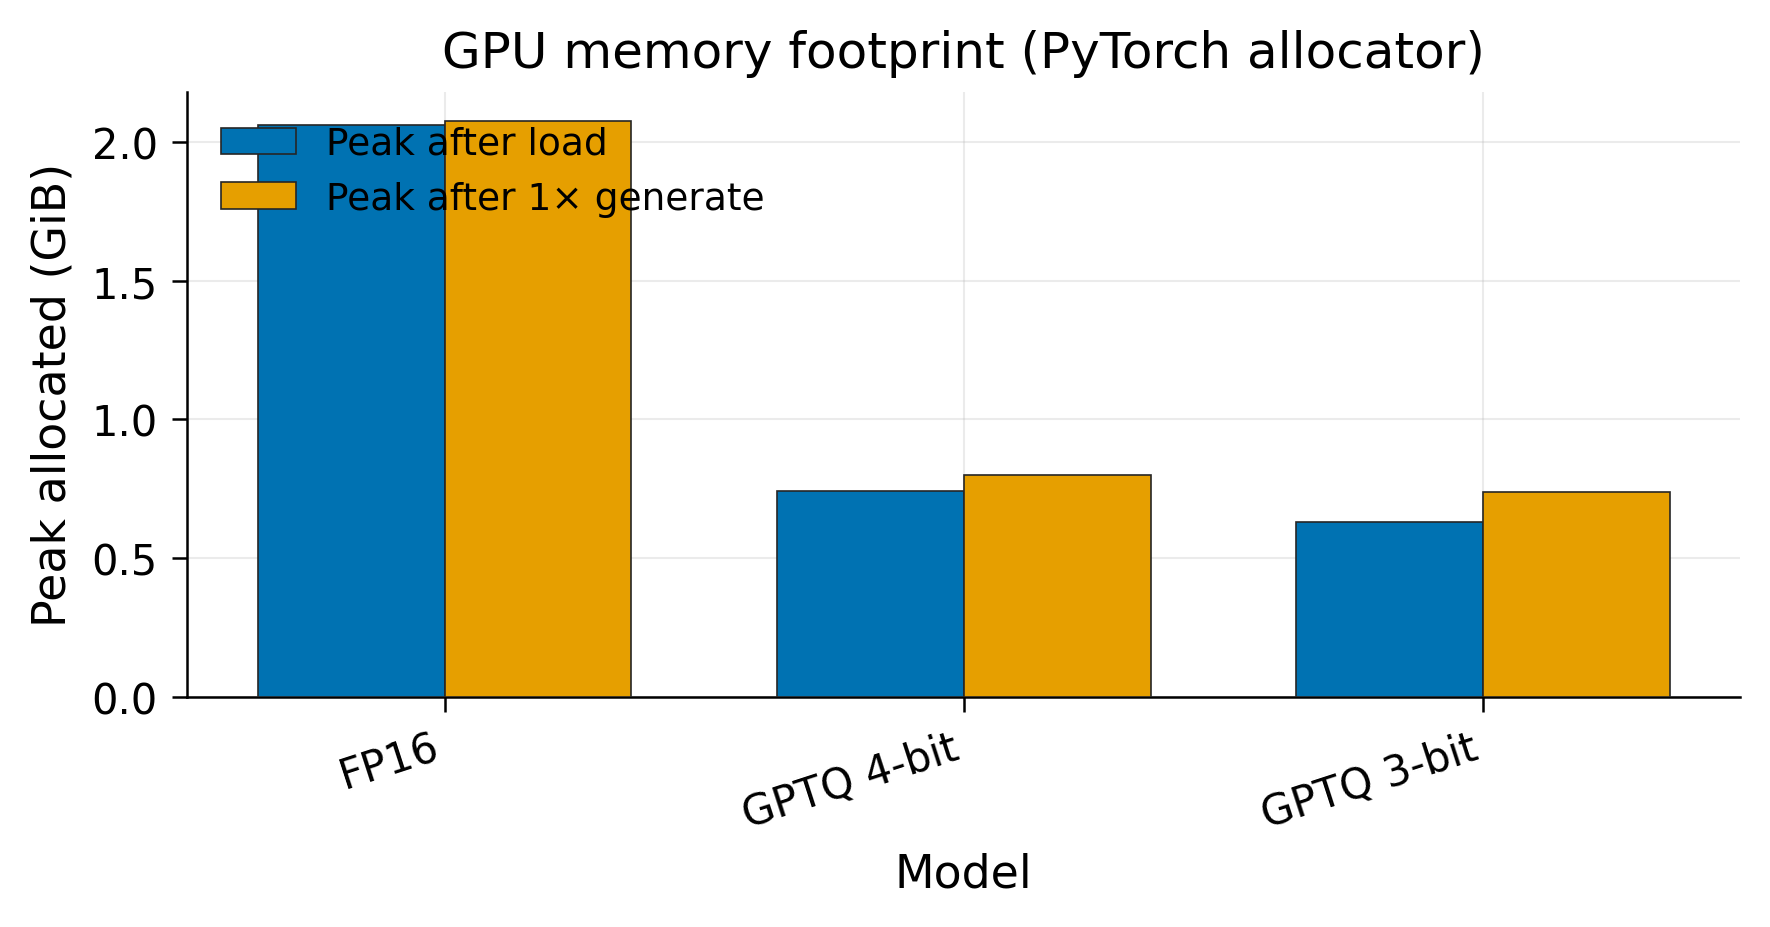
\includegraphics[width=0.85\linewidth]{memory_usage.png}%
  }{%
    \fbox{\parbox[c][0.22\textheight]{0.85\linewidth}{\centering
      \vfill
      \textit{Placeholder: \texttt{results/figures/memory\_usage.png}}
      \vfill
    }}%
  }
  \caption{Peak allocated GPU memory after model load and after one \texttt{generate()} call.}
  \label{fig:memory}
\end{figure}

% ---------------------------------------------------------------------------
% Final tables populated from generated benchmark CSVs.
% ---------------------------------------------------------------------------

\begin{table}[t]
  \caption{WikiText-2 test perplexity (lower is better), from \texttt{results/csv/perplexity\_results.csv}.}
  \label{tab:ppl}
  \centering
  \small
  \begin{tabular}{lc}
    \toprule
    \textbf{Model} & \textbf{Perplexity} \\
    \midrule
    FP16 (baseline)      & 7.40 \\
    GPTQ 4-bit           & 8.04 \\
    GPTQ 3-bit           & 16.15 \\
    \bottomrule
  \end{tabular}
\end{table}

\begin{table}[t]
  \caption{Greedy decoding throughput on a shared prompt (higher tok/s is better), from \texttt{results/csv/speed\_results.csv}.}
  \label{tab:speed}
  \centering
  \small
  \begin{tabular}{lc}
    \toprule
    \textbf{Model} & \textbf{Tokens/s} \\
    \midrule
    FP16      & 43.72 \\
    GPTQ 4-bit & 6.44 \\
    GPTQ 3-bit & 2.62 \\
    \bottomrule
  \end{tabular}
\end{table}

\begin{table}[t]
  \caption{Peak GPU memory usage in GiB from \texttt{results/csv/memory\_results.csv} (lower is better).}
  \label{tab:memory}
  \centering
  \small
  \begin{tabular}{lc}
    \toprule
    \textbf{Model} & \textbf{Peak GPU memory (GiB)} \\
    \midrule
    FP16      & 2.076 \\
    GPTQ 4-bit & 0.799 \\
    GPTQ 3-bit & 0.739 \\
    \bottomrule
  \end{tabular}
\end{table}


\section{Analysis}
\paragraph{Perplexity vs.\ bit-width.}
The measured WikiText-2 perplexities are $7.40$ (FP16), $8.04$ (GPTQ 4-bit), and $16.15$ (GPTQ 3-bit).
Thus, GPTQ 4-bit preserves language modeling quality reasonably well relative to FP16
($+0.64$ absolute PPL), while GPTQ 3-bit introduces a large degradation (more than $2\\times$ FP16 perplexity),
consistent with stronger information loss at 3-bit quantization~\citep{frantar2023gptq}.

\paragraph{Throughput.}
Throughput results are $43.72$ tok/s (FP16), $6.44$ tok/s (GPTQ 4-bit), and $2.62$ tok/s (GPTQ 3-bit).
Contrary to the common expectation that low-bit inference is always faster, both quantized variants are slower on this
Windows setup. The key reason is kernel maturity: on Linux, highly optimized low-bit kernels (often Triton- or
vendor-specific) can outperform FP16, but on Windows with our pinned compatibility stack these optimized paths are limited
or unavailable. As a result, quantized execution can become dequantization- and memory-movement-bound, reducing effective
decode throughput despite smaller weights. This highlights that ``quantization'' and ``quantized acceleration'' are
separate engineering problems.

\paragraph{Memory.}
Peak GPU memory drops from $2.076$\,GiB (FP16) to $0.799$\,GiB (GPTQ 4-bit) and $0.739$\,GiB (GPTQ 3-bit).
This corresponds to approximately $61.5\\%$ and $64.4\\%$ memory reduction versus FP16, respectively.
Therefore, even when throughput regresses on Windows, GPTQ delivers a strong deployment benefit by enabling models
to fit into substantially smaller VRAM budgets and reducing OOM risk.

\paragraph{Threats to validity.}
Windows toolchains differ from Linux CI clusters; disabling Triton changes kernel choices.
TinyLlama is small relative to frontier models; conclusions may not transfer to 7B--70B scales without re-verification.

\section{Conclusion}
We presented an end-to-end, reproducible comparison of FP16 and GPTQ (3/4-bit) quantization for TinyLlama,
evaluating WikiText-2 perplexity, decoding throughput, and GPU memory on a consumer Windows + CUDA stack.
When environment compatibility allows, AWQ is included as an additional comparison arm.
Our final measurements show a clear trade-off: GPTQ yields major memory savings (up to $64.4\\%$) but, under current
Windows kernel constraints, incurs substantial speed penalties relative to FP16.
The accompanying codebase standardizes calibration, evaluation, and plotting for one-command reproduction.
Future work includes scaling to larger models, measuring downstream task accuracy (MMLU, GSM8K),
improving Windows low-bit kernel support, and exploring mixed-precision schemes that combine outlier preservation with
sub-4-bit bulk weights.

\section*{Team Contributions}
\textit{Instructional / course report placeholder---edit to match your course policy.}
\begin{itemize}
  \item \textbf{Member A:} quantization pipelines (GPTQ/AWQ), environment and dependency pinning.
  \item \textbf{Member B:} perplexity evaluation, sliding-window metric verification.
  \item \textbf{Member C:} speed and memory benchmarks, CUDA timing methodology.
  \item \textbf{Member D:} plotting, report writing, literature survey.
\end{itemize}

\section*{Acknowledgments}
We thank the authors of TinyLlama, AutoGPTQ, AutoAWQ, and the Hugging Face ecosystem for open models and tooling.
Compute was provided by \placeholder{institution / lab}.

\bibliographystyle{plainnat}
\bibliography{references}

\end{document}
